%%%%%%%%%%%%%%%%%%%%%%%%%%%%%%%%%%%%%%%%%%%%%%%%%%%%%%%%%%%%%%%%%%%%%%%%%%%%%%%%
%2345678901234567890123456789012345678901234567890123456789012345678901234567890
%        1         2         3         4         5         6         7         8

\documentclass[10pt, conference]{IEEEtran}

%\overrideIEEEmargins                                      % Needed to meet printer requirements.

%In case you encounter the following error:
%Error 1010 The PDF file may be corrupt (unable to open PDF file) OR
%Error 1000 An error occurred while parsing a contents stream. Unable to analyze the PDF file.
%This is a known problem with pdfLaTeX conversion filter. The file cannot be opened with acrobat reader
%Please use one of the alternatives below to circumvent this error by uncommenting one or the other
%\pdfobjcompresslevel=0
%\pdfminorversion=4

% See the \addtolength command later in the file to balance the column lengths
% on the last page of the document

% The following packages can be found on http:\\www.ctan.org
\usepackage{graphicx}
%\usepackage{graphics} % for pdf, bitmapped graphics files
%\usepackage{epsfig} % for postscript graphics files
%\usepackage{mathptmx} % assumes new font selection scheme installed
%\usepackage{times} % assumes new font selection scheme installed
\usepackage{amsmath} % assumes amsmath package installed
\usepackage{amssymb}  % assumes amsmath package installed
\usepackage{bm} % for bold symbols in math mode
\usepackage{cite}

\title{\LARGE \bf
Report: SLIP models for controlling articulated robotic legs
}


\author{Stefan Schneyer and Fabian Kolb}

\begin{document}
\maketitle
\thispagestyle{empty}
\pagestyle{empty}


%%%%%%%%%%%%%%%%%%%%%%%%%%%%%%%%%%%%%%%%%%%%%%%%%%%%%%%%%%%%%%%%%%%%%%%%%%%%%%%%
%\begin{abstract} TODOabstract \end{abstract}

\section{Introduction}
\label{sec:Introduction}


Bio inspired robotics and especially humanoid robots play an increasing role in society and science. Robotic solutions with a structural 
similarity to humans are especially suitable for tasks which are up to now mainly solved by humans. For moving in challenging terrain with higher velocities
hopping is an interesting approach. For simplicity hopping can be simulated with one leg. SLIP models describe the spring-like leg behaviour
of animals and humans in a very simple and abstract way. The model reduces the leg to a massless spring with a point mass attached to the top. 
This abstract SLIP model behaviour is then projected on the dynamics of an articulated leg. 
In a first stage a closed loop dynamics is generated based on the SLIP model. In the second stage the high order robotic leg tracks this closed loop dynamics 
and uses a feedback controller to adapt to deviations. The robot state is modelled as automaton. A continuous state captures the position of the 
robot in the 3D space, the hip angle and knee angle. A discrete state models the transition of flight to stance and stance to flight phase. 
A control structure is implemented for both the flight and the stance phase. 
For the flight phase a cascade control consisting of PI and PID controller is used. When touching the ground, the SLIP dynamics can be 
projected onto the CoG motion of the robotic leg. From there the joint actuator torques which are necessary to generate the operational space 
forces is calculated. Real robotic legs differ from the simplified SLIP model because the mass and inertia of the leg's segments influence the 
the robot's motion. Real robots suffer from the impact when the foot strikes the ground. This leads to a loss of kinetic energy which is incorperated in 
the SLIP model by an energy compensation. Different types of integration are implemented in order to study their effect on the controller stability. 
The project is implemented in Python. The RBDL library is used, which offers efficient rigid body dynamics algorithms. 
For visualization Meshup, a tool that was developed with RBDL is used.




\section{SLIP model}
\label{sec:SLIP model}
The SLIP model is an abstraction capturing the locomotion behavior of robots with light, compliant legs. In this model the body is reduced to a point mass \( m \). The
leg is represented by a massless spring with stiffness \({k}_0 \) and a rest length \({l}_0 \). For this system the equations of motion are the following:
\begin{equation}
   \begin{bmatrix} m & 0 \\ 0 & m \end{bmatrix}
   \begin{bmatrix} \ddot{x} \\ \ddot{y} \end{bmatrix}
   +
   \begin{bmatrix} 0 \\ mg \end{bmatrix}
   =
   \begin{bmatrix} {F}_{x} \\ {F}_{y} \end{bmatrix},
   \label{eq:equation of motion}
\end{equation}

where x and y are the coordinates of the center of mass (COM). \({F}_x \) and \({F}_y \) are the ground reaction forces (GRF). The GRFs are 0 during flight and depend 
on the length of the spring \(l\) during compression and the landing angle \(\alpha\) of the foot.

\begin{equation}
   \begin{bmatrix} {F}_{x}  \\ {F}_{y}  \end{bmatrix}
   =
   {k}_{0} ({l}_{0} -l)
   \begin{bmatrix} -cos(\alpha) \\ sin(\alpha) \end{bmatrix},
\end{equation}

The SLIP model describes running as a series of apex heights \({y}_i \)

\begin{figure}[h]
   \centering
   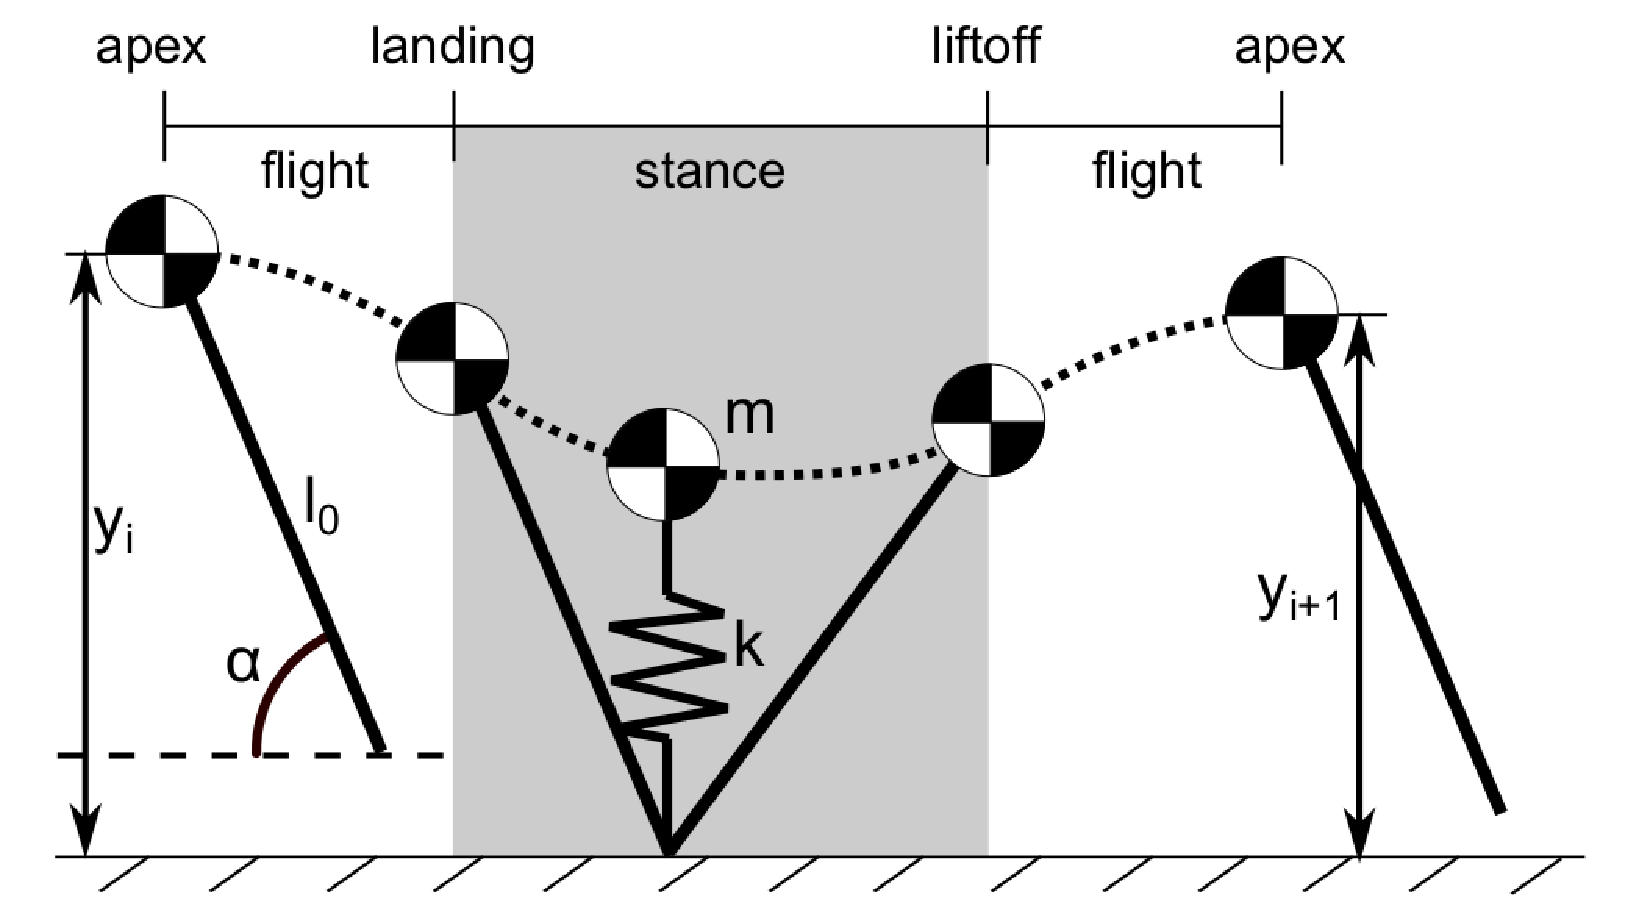
\includegraphics[scale=0.2]{"assets/SMM2.pdf"}
   \caption{flight and stance phases of SLIP model \cite{Wu2014}}
   \label{fig_SLIP_phase}
\end{figure}


In Fig. \ref{fig_SLIP_phase} it becomes clear how the robot trajectory can be separated in flight and stance phases. The gait behavior is characterized by the forward speed and the apex height.
The SLIP model is a conservative system without any friction or other mechanism to dissipate the dynamics, and thus, their phase space does not shrink over time. 
Therefore, the apex height and forwards speed are coupled through the system energy and the trajectory is fully characterized by the apex height. 
The transition between two consecutive apex heights is defined by the landing angle \(\alpha\):
\begin{equation}
   {f}_{yi+1}={f}_{yi}|(\alpha),
\end{equation}
The landing angle is used to achieve deadbeat stability of the system \cite{Wu2014} \cite{Hutter2010}.




\section{Control}
\label{sec:Control}
Different control designs were used for the flight and stance phase. 

\subsection{Stance control}
The mechanics of a robotic leg under support conditions are the following:
\begin{equation}
   M(q)\ddot{q}+b+g+{J}_{s}^{T}+F_{s}=S^{T}+{\tau},
\end{equation}

with the mass matrix M , the coriolis and centrifugal force vector b , the gravitational force g , the ground contact force
Fs, the corresponding support Jacobian \({J}_{s}\), the actuation torques \(\tau = [{\tau}_{Hip}, {\tau}_{Knee}]^{T}\) and the actuator selection matrix S
limiting the actuation to hip and knee joints. The generalized coordinates  \(q = [x_{FloatingBase}, y_{FloatingBase}, {\phi}_{Hip}, {\phi}_{Hip}]^{T}\)
describe the current robot state. Since we assume no slip between foot and ground during contact. The following conditions apply: 
\begin{equation}
   \dot{x}_{s} = J_{s} \dot{q} = 0,
\end{equation}
\begin{equation}
   \ddot{x}_{s} = J_{s} \ddot{q} + \dot{J}_{s} \dot{q}=0,
\end{equation}

This reduces the mechanics of a robotic leg to a support consistent description:
\begin{equation}
   M \ddot{q} + {N}_{s}^{T}(b + g) + {J}_{s}^{T} {\Lambda}_{s} {\dot{J}}_{s} \dot{q} = {(S {N}_{s})}^{T} \tau,
\end{equation}

with the support inertia Matrix \({\Lambda}_{s} = {({J}_{s} {M}^{-1} {J}_{s}^{T})}^{-1}\) and the support nullspace 
\({N}{s}=[I-{M}^{-1} {J}_{s}^{T} {\Lambda}_{s} {J}_{s}]\). The real articulated leg has inertia and mass in each leg segment. Therfore it is affected 
by the impulse of the foot hitting the ground. The change of the generalized velocity is described by the nullspace \({\dot{q}}^{+}={N}_{s} {\dot{q}}^{-}\)
The stance dynamics can now be projected on the center of gravity (CoG) of the articulated leg. This allows to compute the operational space force F:
\begin{equation}
   \Lambda {\ddot{r}}_{CoG} + {\mu}^{*} + {p}^{*} = F, 
   \label{eq:operational space force F}
\end{equation}
The operational space force F do relate to the robot actuation like the following:
\begin{equation}
   \tau = {J}^{*T}F,
\end{equation}

The different terms which are used in \ref{eq:operational space force F} are presented in the follwing:\\* 
i) task interia: 
\begin{equation}
   {\Lambda}^{*} = {(J {M}^{-1} S {N}_{s} {J}^{*})}^{-1}, 
\end{equation}
ii) projected coriolis and centrifugal terms
\begin{equation}
\begin{aligned}
   {\mu}^{*} = & \ {\Lambda}^{*} {J}_{CoG} {M}^{-1} {N}_{s}^{T} b - {\Lambda}^{*} {\dot{J}}_{CoG} \dot{q} \\
   & \ + {\Lambda}^{*} {J}_{CoG} {M}^{-1} {J}_{s}^{T} {\Lambda}_{s} {\dot{J}}_{s} {\dot{q}}_{CoG},\
\end{aligned}
\end{equation}
iii) projected gravitational term
\begin{equation}
   {p}^{*} = {\Lambda}^{*} {J}_{CoG} {M}^{-1} {N}_{s}^{T} g,
\end{equation}
iv) support reduced Jacobian
\begin{equation}
   {J}^{*} = {J}_{CoG} {M}^{-1} {(S {N}_{s})}^{T} {(S {N}_{s} {M}^{-1} {(S {N}_{s})}^{T})}^{-1}
\end{equation}

After projecting the stance dynamics of the robotic leg onto the CoG, the SLIP dynamics can now also be imposed onto the CoG. Then the equations of motion of the SLIP model 
in \ref{eq:equation of motion} can be solved for the \(\ddot{x}, \ddot{y}\) which are then be inserted for \({\ddot{r}}_{CoG}\) in \ref{eq:operational space force F}. This 
enables the SLIP control law:
\begin{equation}
   \tau = {J}^{*T} ({\Lambda}^{*} \frac{1}{m} ({F}_{leg} + mg) + {\mu}^{*} + {p}^{*})
\end{equation}
If we assume to have an perfect model of the articulated leg and the CoG motion of the SLIP model is feasible, using the SLIP control law the CoG of the articulated leg will 
follow the SLIP trajectory accuratly. The paragraph follows Hutters work in \cite{Hutter2010}


\subsection{Flight control}
A cascade control is used in the flight phase to track the landing angle \(\alpha\). The cascade control consists of two PI and one PID controller and is shown in Fig \ref{fig:cascade}. 
The position controller uses the difference of the goal and current position of the CoG to calculate the desired velocity of the CoG. The velocity controller uses 
the difference of the goal and current velocity of the CoG to calculate the desired angle of attack in the SLIP model. From this angle the goal foot position can be 
calculated. This foot position is compared with the current foot position of the acrticulated leg and a desired acceleration of the foot is set. From there the torques 
required to generate these accelerations of the robot foot are estimated. The relation between joint accelerations and end-effector accelerations is given by the 
Jacobians. To transform the the accelerations in the joints to actuations the mass matrix and Newton's first law is used.

\begin{figure}[h]
   \centering
   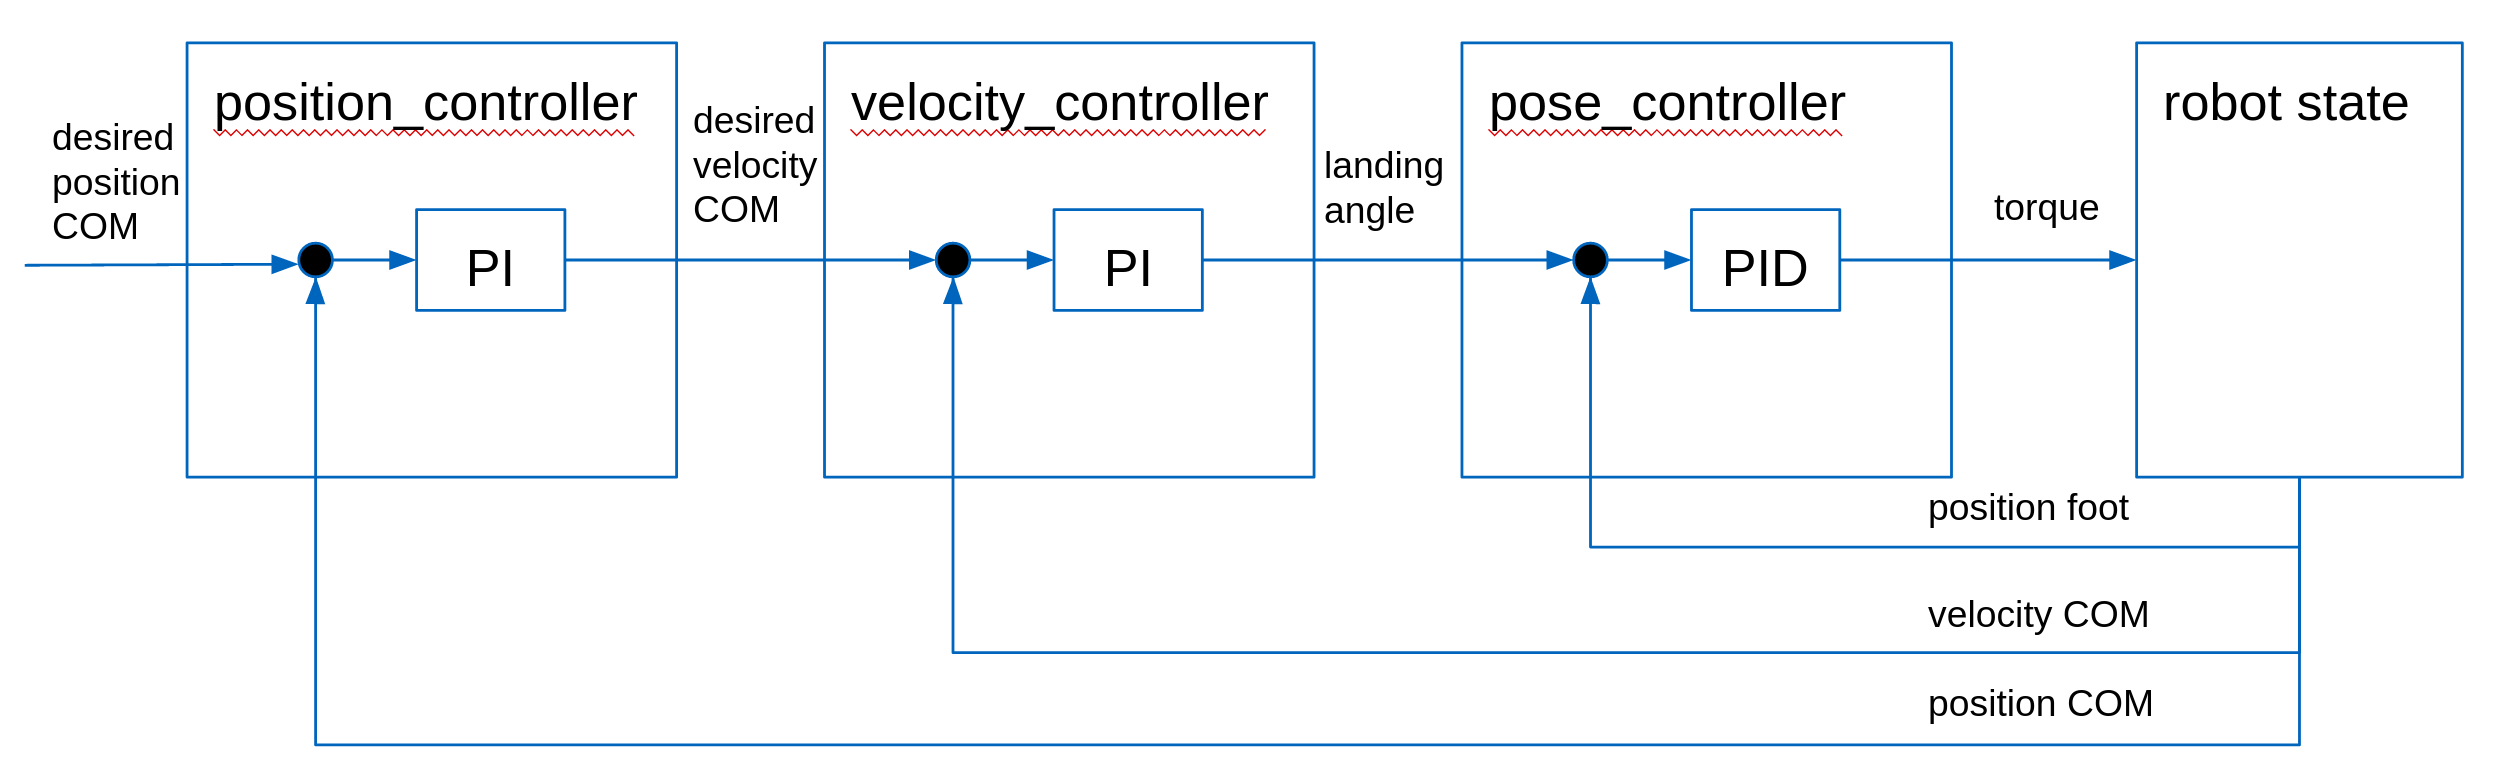
\includegraphics[scale=0.11]{"assets/cascade.png"}
   \caption{Flight control}
   \label{fig:cascade}
\end{figure}

\section{SLIPic}
\label{sec:SLIPic}
For the SLIP model the leg is modeled with a masseless spring. In reality the articulated leg does have a mass and inertia for each segment. The impact when the foot strikes the ground 
therefor influences the velocity of the articulated leg. Therfore the generalized velocity changes through the impact. Like mentioned earlier this velocity change is described throught 
the support nullspace. This velocity change leads to a loss of kinetic energy:
\begin{equation}
\begin{aligned}
   \Delta E = & \ 0.5 {m}_{CoG} ({|{\dot{r}}_{CoG}^{-}|}^{2} - {|{\dot{r}}_{CoG}^{+}|}^{2}) \\
   & \ =0.5 {m}_{CoG} {\dot{q}}^{-T} ({J}_{CoG}^{T} {J}_{CoG} - \\
   & \ {N}_{s}^{T} {J}_{CoG}^{T} {J}_{CoG} {N}_{s}) {\dot{q}}^{-},
\end{aligned}
\end{equation}

The SLIP model does not account for that energy loss. If the normal SLIP model is used for the SLIP 
control law in the stance phase this energy loss is not compensated. The potential energy is reduced by the loss of kinetic energy in every jump. This leades to a reduced apex height 
in every foot strike. To prevent that an extended SLIP model is used which considers the loss of kinetic energy through the impact. This model is called SLIP with impact compensation 
(SLIPic). In this model the spring of the SLIP model is pre-compressed at the landing such that the loss of kinetic energy in the articulated leg equals the energy stored in the spring: 

\begin{equation}
   \Delta E = 0.5 k {\Delta l}^{2},
\end{equation}

The spring forces in the SLIP model and thefore also the ground reaction forces (GRF) in the articulated leg are increased such that the energy loss is compensated and the apex height is 
held constant. Fig \ref{fig:SLIPic} visualizes how the virtual spring energy copnesates the loss of kinetic energy.

\begin{figure}[h]
   \centering
   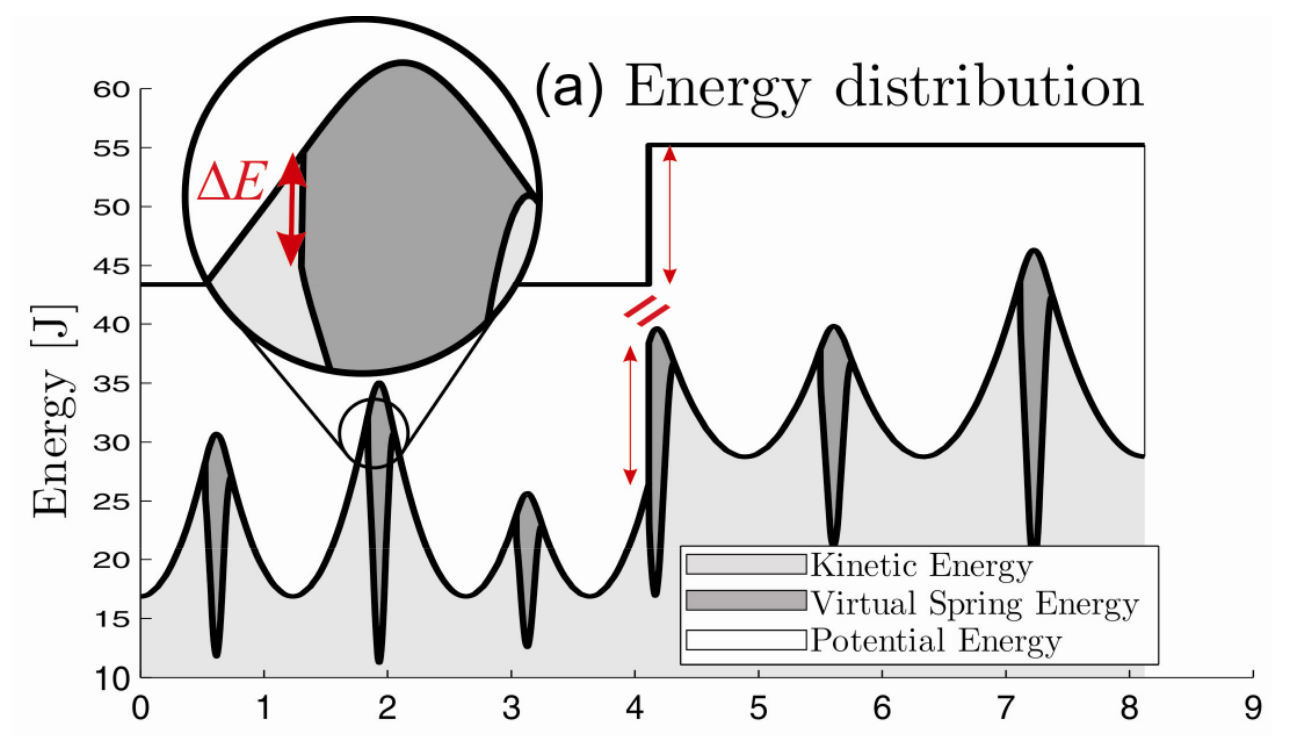
\includegraphics[scale=0.15]{"assets/SLIPic.png"}
   \caption{impact compensation in SLIPic \cite{Hutter2010}}
   \label{fig:SLIPic}
\end{figure}

\section{Structure}
\label{sec:Structure}
\subsection{Hybrid Automaton}
\subsection{Implementation}

\section{Solver}
\label{sec:Solver}
The calculate the robots state we iteratively do a control, forward dynamics and integration step. In the control step we calculate the requred robot actuation from 
the current robot state. For this we use our stance and flight controller described in Section \ref{sec:Control}. In teh forward dynamics the robot state derivative 
is calculated from the current robot state and the robot actuation. Integrating this robot state derivative returns the robot state for the next time step. The step size 
of the solver loop determines the accuracy of the solution for the robot state. The step size is derermined by the steps the integrator takes.


\begin{figure}[h]
   \centering
   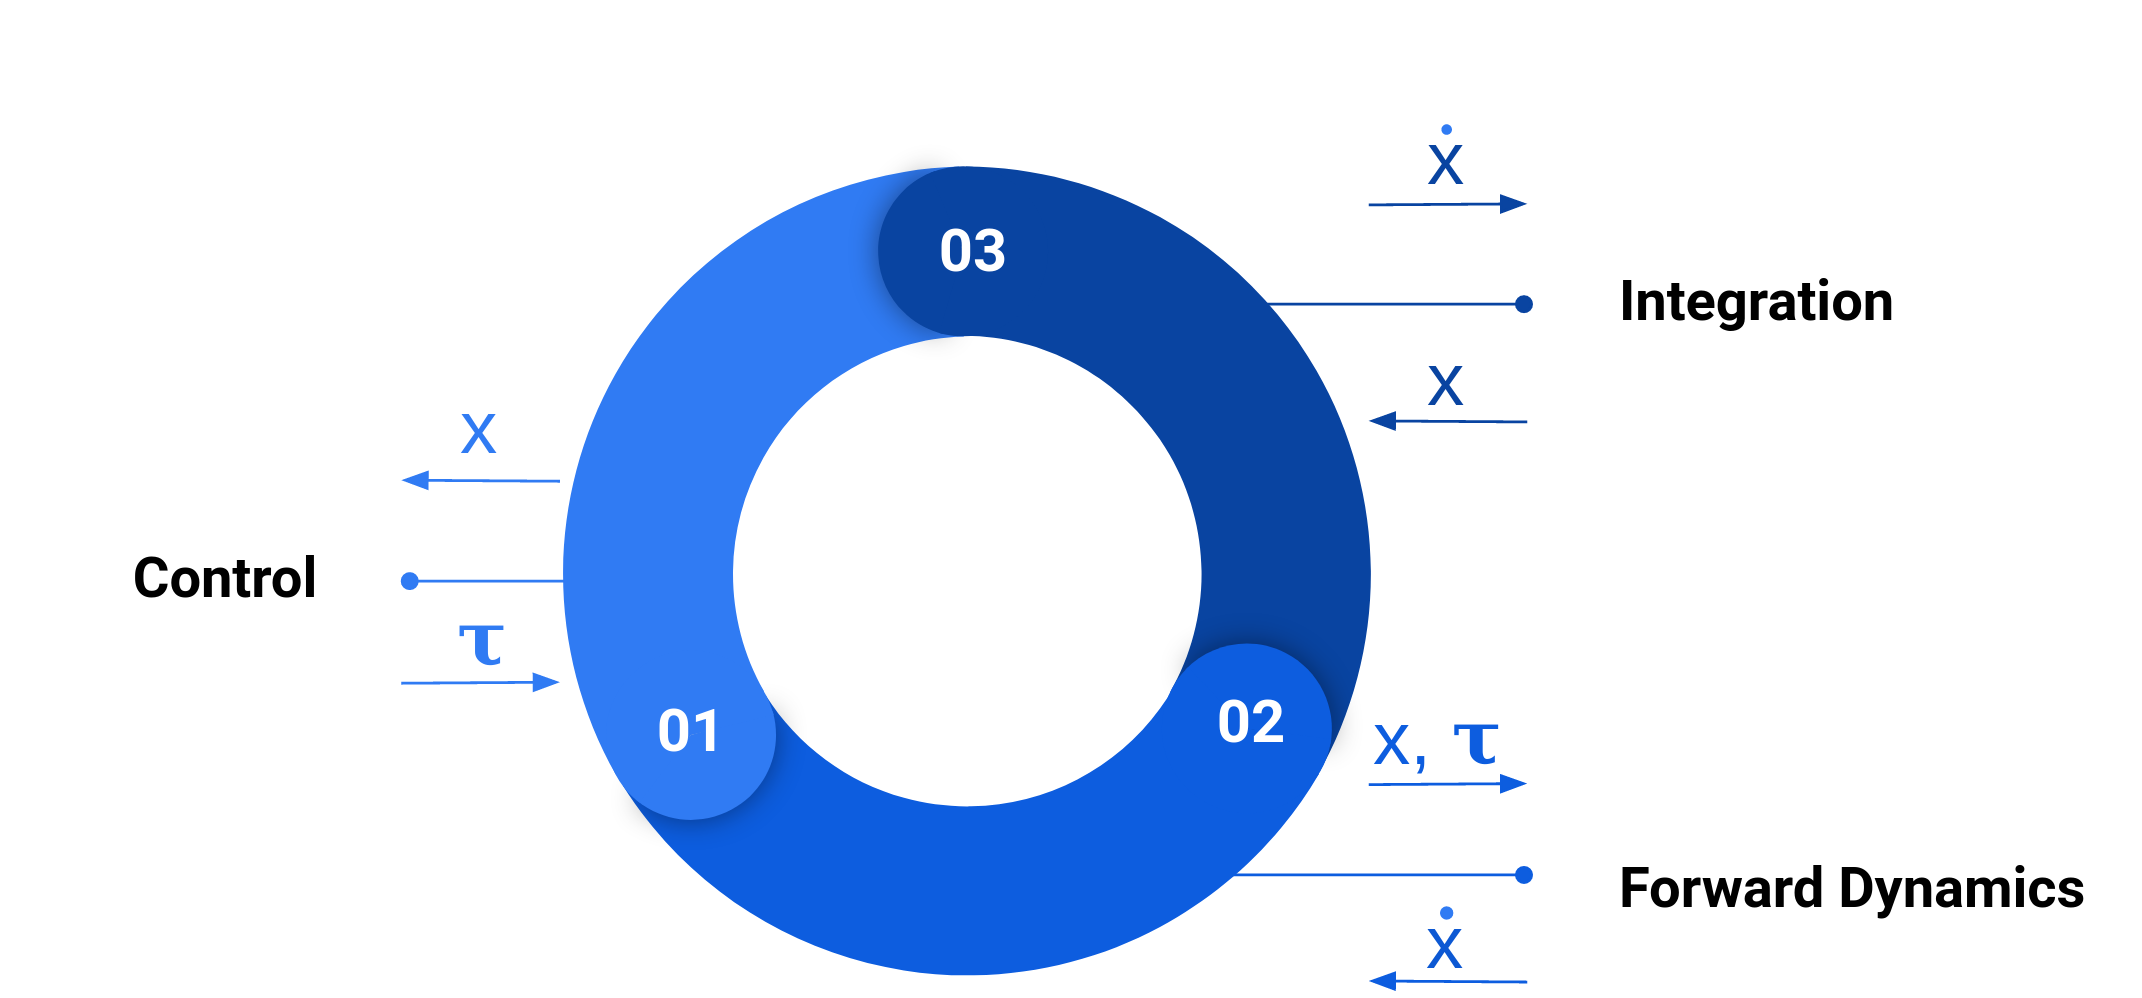
\includegraphics[scale=0.12]{"assets/solver_iteration.png"}
   \caption{Solver iteration}
   \label{fig:solver_iteration}
\end{figure}

In each iteration a state transition from stance to flight or flight to stance phase is checked. The jump function uses the solved robot state from this iteration 
for the discrete state transition. 
In a first attempt the ivp solver by SciPy is applied. This solver uses the Runge-Kutta method of order 5(4) to numerically integrate a system of ordinary differential 
equations given an initial value. The robot state derivative i is integrated until the end of the integration interval is reached or an event function is 
fullfilled.  The guard functions which mark the transition between the discrete states are used as event functions. The ivp solver will find an accurate robot state 
at time t when the event function is zero. This has the advantage that the robot state is known exactly at the state transition and can be used in the jump function. 
The ivp solver uses variable step size for each integration step. This variable step size causes unstable behaviour in the system. The PID controller in the 
flight control numerically differentiates the foot position error. A differentiation with a variable step size might cause problem and makes 
it hard to tune the PID controller. Fig \ref{fig:ivp solver} shows that after 4 jumps the system becomes unstable.

\begin{figure}[h]
   \centering
   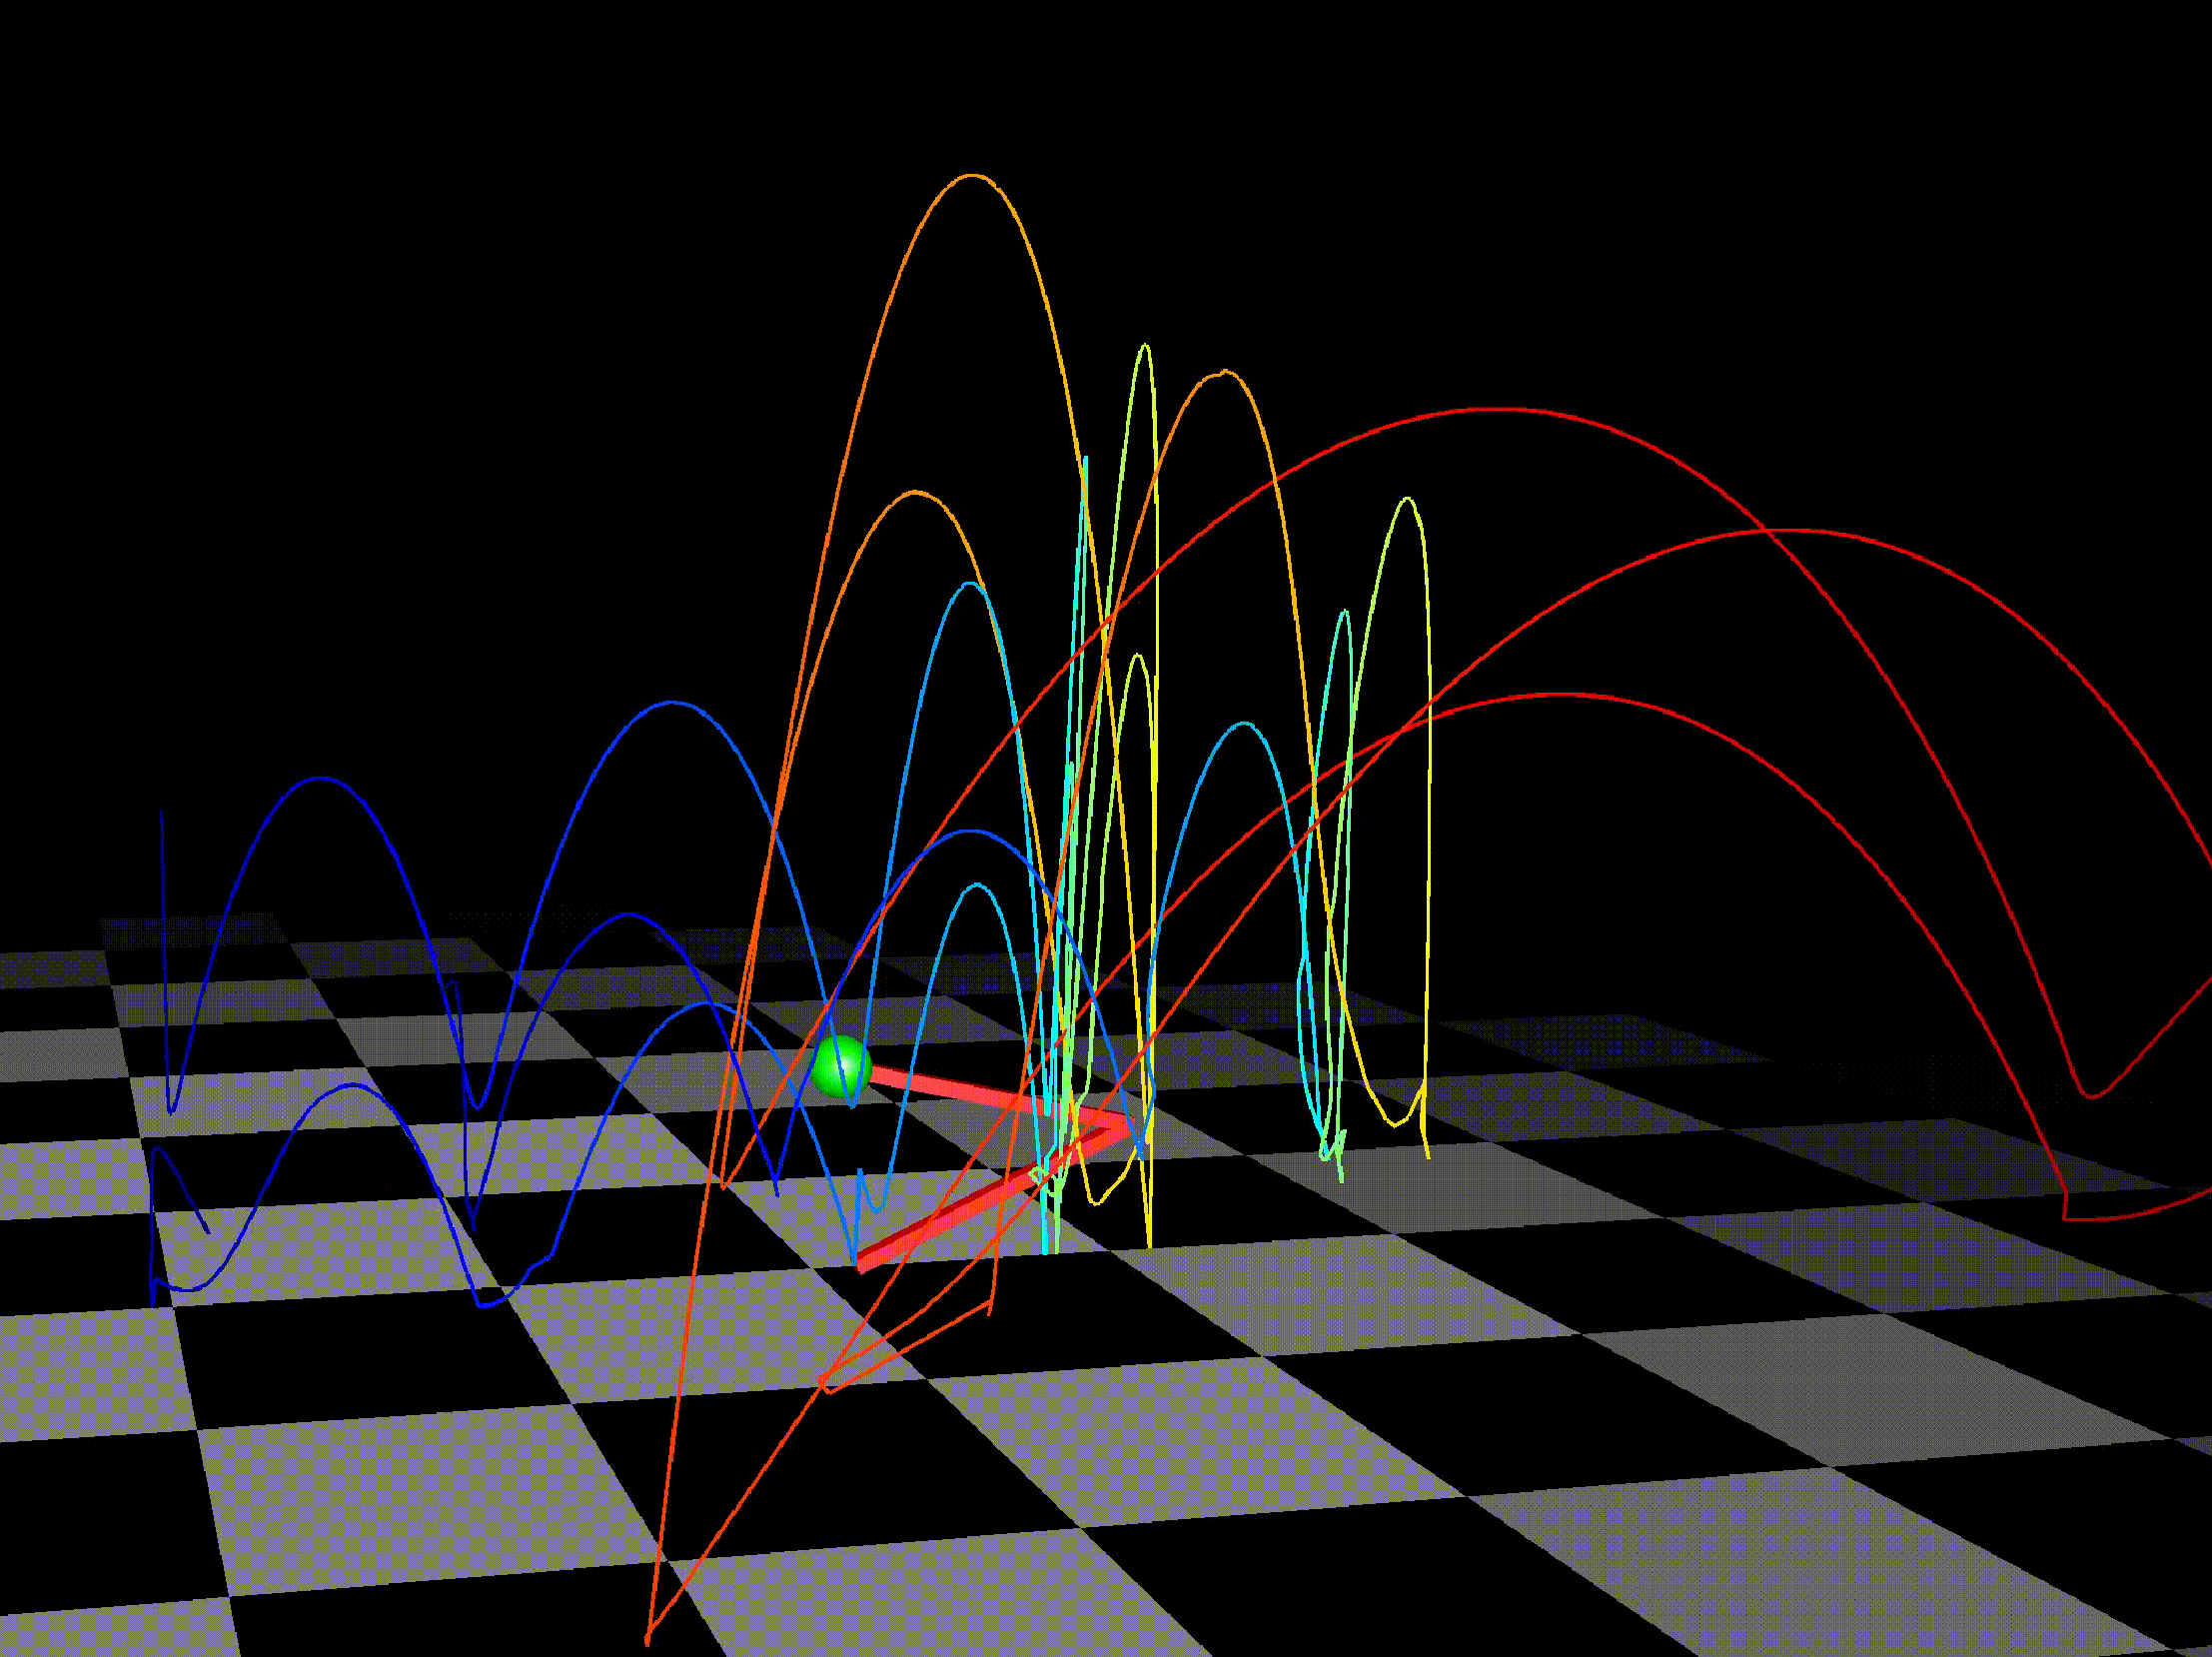
\includegraphics[scale=0.11]{"assets/solver_ivp.png"}
   \caption{ivp solver}
   \label{fig:ivp solver}
\end{figure}

In a second attempt the Runge-Kutta method of order 5(4) with a fixed step size is evaluated. This has the disandvatage that no root-finding is used. After each 
integration step the guard functions are checked to make sure whether a discrete state transition did occur. Compared to the ivp solver the robot state at the 
transition is not as accurate with this integration method. Choosing a small enough step size makes this problem insignificant. The fixed step size helps a lot 
to make the flight controller more stable. Fig \ref{fig:RK45 solver} shows the good results with this method.

\begin{figure}[h]
   \centering
   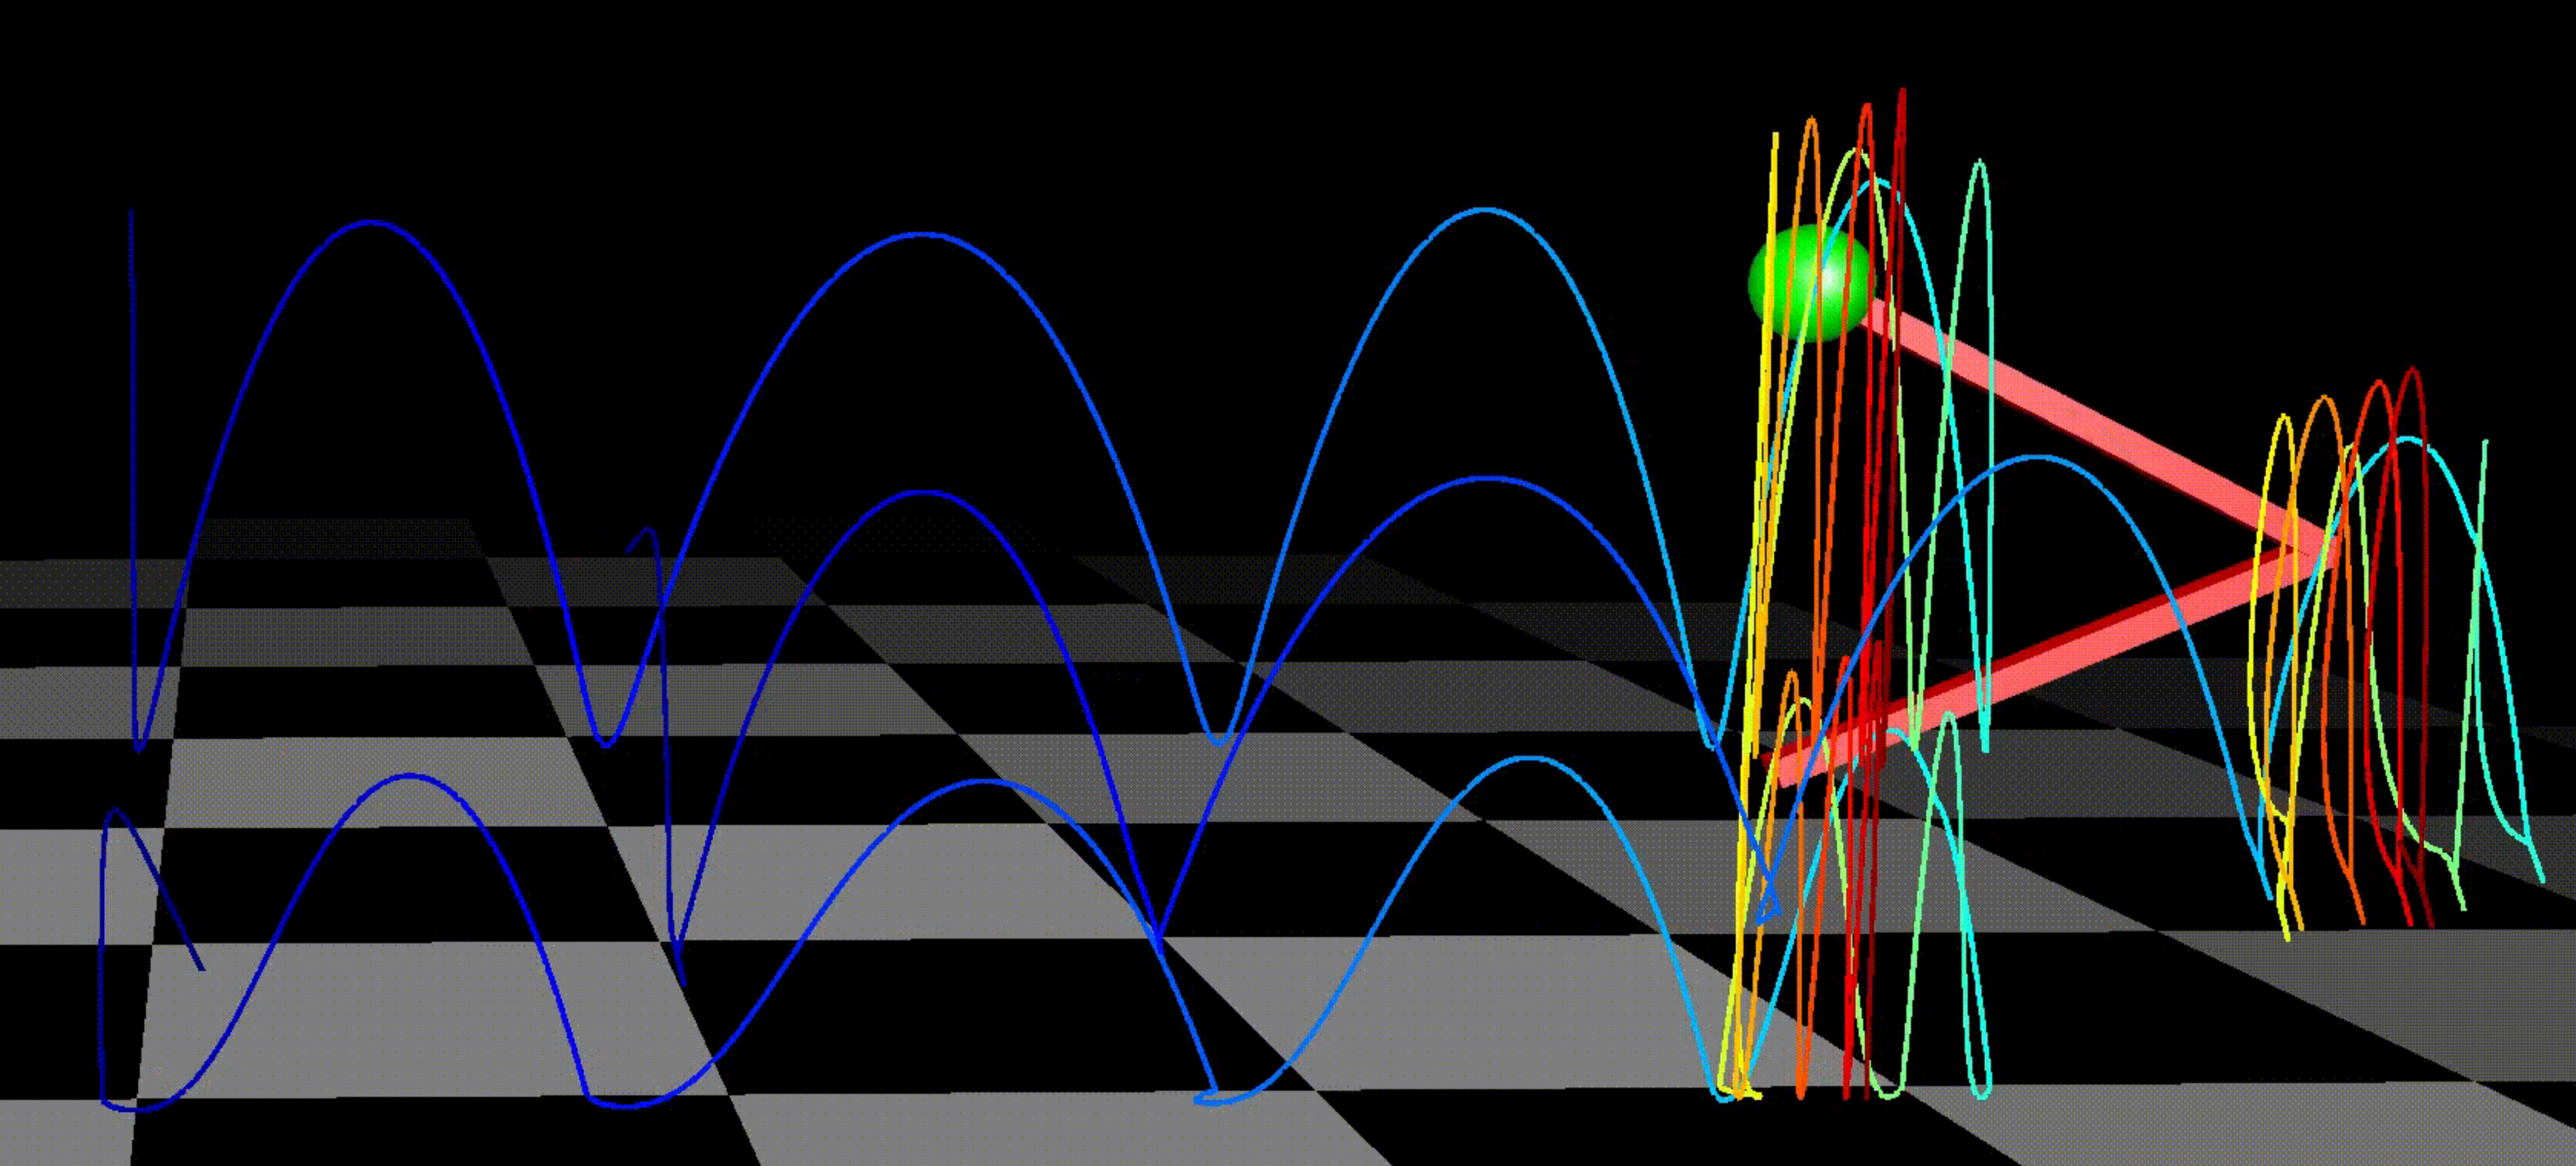
\includegraphics[scale=0.074]{"assets/solver_rk45.png"}
   \caption{RK45 solver}
   \label{fig:RK45 solver}
\end{figure}

\section{Conclusion}

\addtolength{\textheight}{-12cm}   % This command serves to balance the column lengths
                                  % on the last page of the document manually. It shortens
                                  % the textheight of the last page by a suitable amount.
                                  % This command does not take effect until the next page
                                  % so it should come on the page before the last. Make
                                  % sure that you do not shorten the textheight too much.

\nocite{*}
\bibliographystyle{IEEEtran}
\bibliography{IEEEabrv, report}

\end{document}
